\chapter{Heap}

\section{Introduction}
Heap-ordered. Binary heap is one of the implementations of Priority Queue (ADT). 

\section{Operations}
Assume the root \textbf{starts} at $a[1]$ rather than $a[0]$.
\\
Basic operations:
\begin{enumerate}
\item sink()/ sift\_down() - recursive
\item swim()/ sift\_up() - recursive
\item build()/ heapify() - bottom-up sink()
\end{enumerate}
\subsection{Sink}
\begin{python}
def sink(self, idx):
    while 2*idx <= self.N:
        c = 2*idx
        if c+1 <= self.N and self.less(c, c+1):
            c += 1
        if not self.less(idx, c):
            return 

        self.swap(idx, c)
        idx = c
\end{python}
\subsection{Swim}
\begin{python}
def swim(self, idx):
    while idx > 1 and self.less(idx/2, idx):
        pi = idx/2
        self.swap(pi, idx)
        idx = pi
\end{python}
\subsection{Heapify}
Worst case: Heapifying \textbf{a sorted array} is the worst case for heap construction, because the root of each subheap considered sinks all the way to the bottom. The worst case complexity $\sim 2N$.

Building a heap is O(N) rather than $O(N \lg N)$.

Proof:
\begin{eqnarray*}
&& \because \sum_{i=0}^{+\infty} {ix^i} =\frac{x}{(1-x)^2} \\
&& \therefore \sum_{h=0}^{\lfloor\lg n\rfloor}{\Big\lceil\frac{n}{2^{h+1}}\Big\rceil
O(h)} = O\Bigg(n\sum_{h=0}^{\lfloor\lg n\rfloor}{\frac{h}{2^h}}\Bigg) \\
&& \therefore \sum_{h=0}^{\lfloor\lg n\rfloor}{\Big\lceil\frac{n}{2^{h+1}}\Big\rceil
O(h)} = O(n)
\end{eqnarray*}

\section{Implementation}
The self-implemented binary heap's index usually starts at 1 rather than 0. 

The array representation of heap is in \textbf{level-order}.

A 3-heap is an array representation (using 1-based indexing) of a complete 3-way tree. The children of $a[k]$ are $a[3k-1]$, $a[3k]$, and $a[3k+1]$.

The main reason that we can use an array to represent the heap-ordered tree in a binary heap is because the tree is \textbf{complete}.

Suppose that we represent a BST containing N keys using an array, with $a[0]$ empty, the root at $a[1]$. The two children of $a[k]$ will be at $a[2k]$ and $a[2k+1]$. Then, the length of the array might need to be as large as $2^N$.

\begin{figure}[hbtp]
\centering
\subfloat{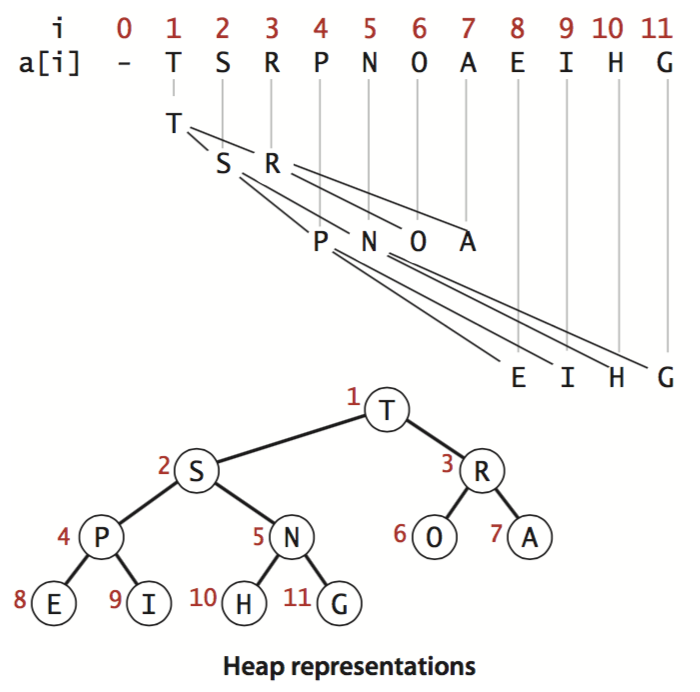
\includegraphics[scale=.90]{heapRepr}}
\caption{Heap representation}
\label{fig:heap} 
\end{figure}

\section{Python Heapq}
Python only has built in min-heap. To use max-heap, you can: 
\begin{enumerate}
\item Revert the number: 1 becomes -1.
\item Wrap the data into another class and override \textbf{comparators}: \_\_cmp\_\_ or \_\_lt\_\_
\end{enumerate}

The following code presents the wrapping method:
\begin{python}
class Value(object):
    def __init__(self, val):
        self.val = val
        self.deleted = False  # lazy delete 

    def __cmp__(self, other):
        # Reverse order by height to get max-heap
        assert isinstance(other, Value)
        return other.val - self.val
\end{python}

Normally the deletion by value in Python is $O(n)$, to achieve $O(\lg n)$ we can use \textbf{lazy deletion}. Before take the top of the heap, we do the following:
\begin{python}
while heap and heap[0].deleted:
    heapq.heappop(heap)
\end{python}
